\documentclass{ComputationalAlgorithmsArticle}

\usepackage[dvips]{graphicx}
\usepackage{float}
\usepackage{subfigure}

\usepackage[dvips,
bookmarks,
bookmarksopen,
backref,
colorlinks,linkcolor={blue},citecolor={blue},urlcolor={blue},
]{hyperref}

\title{Planar Patch Construction}

% 
% NOTE: This is the last number of the "handle" URL that 
% The Insight Journal assigns to your paper as part of the
% submission process. Please replace the number "1338" with
% the actual handle number that you get assigned.
%
\newcommand{\IJhandlerIDnumber}{3303}

% Increment the release number whenever significant changes are made.
% The author and/or editor can define 'significant' however they like.
\release{0.00}

% At minimum, give your name and an email address.  You can include a
% snail-mail address if you like.

\author{David Doria}
\authoraddress{Rensselaer Polytechnic Institute}


\begin{document}

\IJhandlefooter{\IJhandlerIDnumber}


\ifpdf
\else
   %
   % Commands for including Graphics when using latex
   % 
   \DeclareGraphicsExtensions{.eps,.jpg,.gif,.tiff,.bmp,.png}
   \DeclareGraphicsRule{.jpg}{eps}{.jpg.bb}{`convert #1 eps:-}
   \DeclareGraphicsRule{.gif}{eps}{.gif.bb}{`convert #1 eps:-}
   \DeclareGraphicsRule{.tiff}{eps}{.tiff.bb}{`convert #1 eps:-}
   \DeclareGraphicsRule{.bmp}{eps}{.bmp.bb}{`convert #1 eps:-}
   \DeclareGraphicsRule{.png}{eps}{.png.bb}{`convert #1 eps:-}
\fi


\maketitle


\ifhtml
\chapter*{Front Matter\label{front}}
\fi

\begin{abstract}
\noindent

This document presents code to create a mesh of a piece of a plane that is defined by a reasonably planar point set. This is useful when visualizing the output of point cloud segmentation algorithms.

The code is available here:
https://github.com/daviddoria/vtkPlanarPatch

\end{abstract}

\IJhandlenote{\IJhandlerIDnumber}

\tableofcontents
%%%%%%%%%%%%%%%%%%%%
\section{Introduction}
This document presents code to create a mesh of a piece of a plane that is defined by a reasonably planar point set.

\section{Algorithm}
\begin{itemize}
 \item Project the approximately planar 3D points onto their best fit plane
 \item Find a coordinate system on the best fit plane. This is done using the following procedure:
  \begin{itemize}
   \item Find one vector in the plane, $v_0$, by subtracting any two points: $v_0 = p_1 - p_0$. Normalize this vector.
   \item Find a second vector in the plane, $v_1$, by computing the cross product of the plane's normal and $v_0$. Normalize this vector.
   \item Create a set of three points that define a 2D coordinate system (origin and two points unit distance along each of the axes) for the local coordinate system that was just found and for the world coordinate system. For the world coordinate system, these points are simply $(0,0,0)$, $(1,0,0)$, and $(0,1,0)$. For the local coordinate system, they are $p_0$, $(p_0 + v_0)$, and $(p_0 + v_1)$.
  \end{itemize}
 \item Compute the transform from the local coordinate system to the world coordinate system (using a vtkLandmarkTransform).
 \item Compute the 2D Delaunay triangulation on the transformed points. It is not necessary to actually transform the points, the transform can simply be passed to vtkDelaunay2D.
 \item If the user has specified the FlatOutput flag, the topology of the resulting triangulation will be applied to the projected points (the original 3D points projected on their best fit plane) and passed to the output.
 \item If the user has not specified the FlatOutput flag, the topology of the triangulation will be applied to the original 3D points and passed to the output.
\end{itemize}

%%%%%%%%%%%%%%%%%%%%
\section{Demonstration}
In Figure \ref{fig:Demo}, we show the result of the planar patch computation for both FlatOutput and non FlatOutput.
\begin{figure}[H]
\centering
\subfigure[Original, reasonably planar points.]
  {
  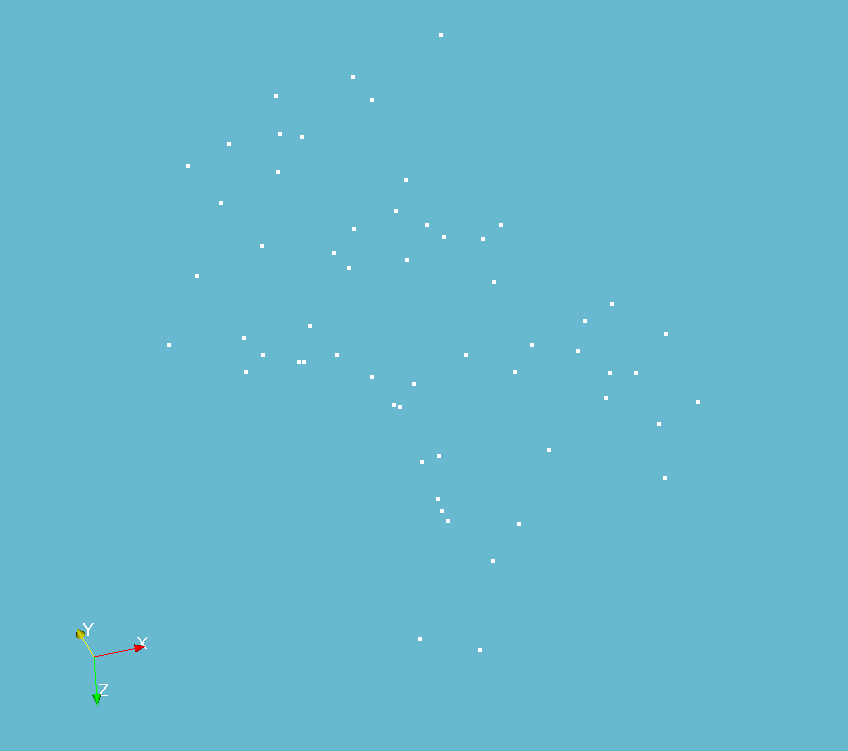
\includegraphics[width=0.3\linewidth]{images/points}
  \label{fig:Demo:Original}
  }
\subfigure[The flat output patch.]
  {
  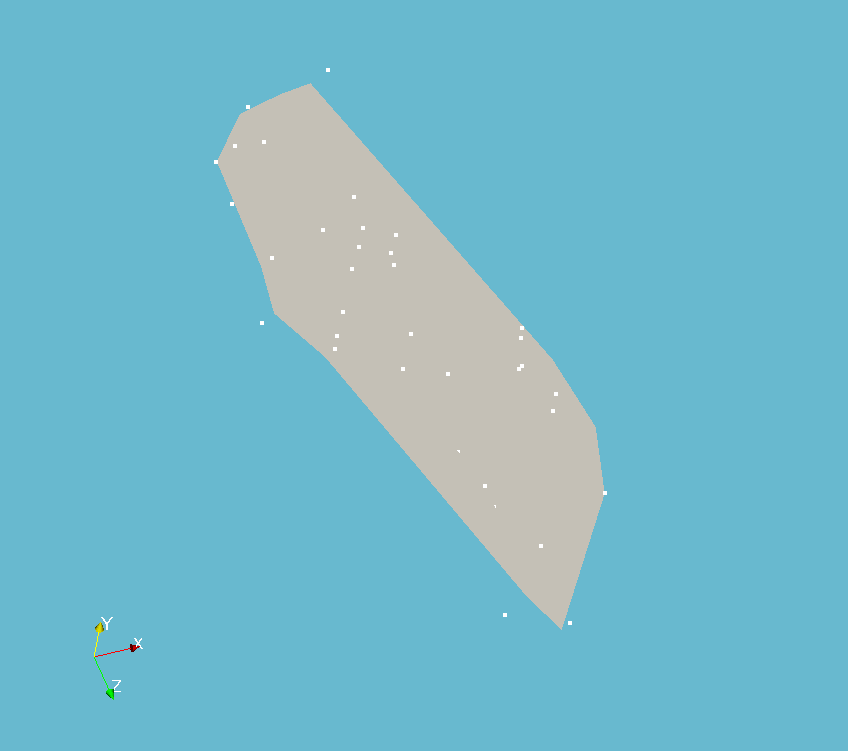
\includegraphics[width=0.3\linewidth]{images/FlatOutput}
  \label{fig:Demo:FlatOutput}
  }
\subfigure[The non flat output patch.]
  {
  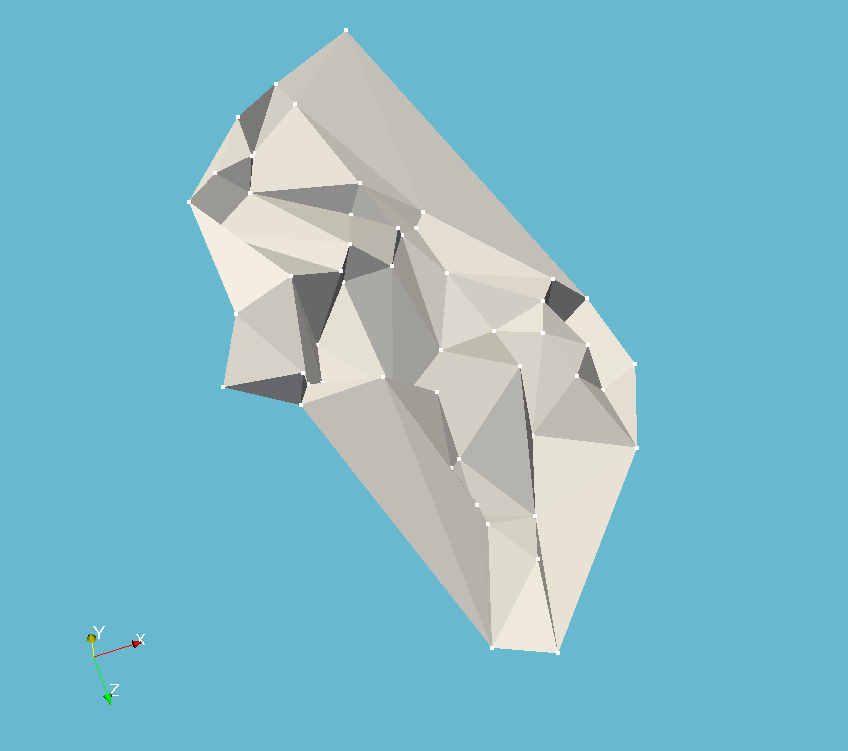
\includegraphics[width=0.3\linewidth]{images/NonFlatOutput}
  \label{fig:Demo:NonFlatOutput}
  }
\caption{Planar patch computation demonstration.}
\label{fig:Demo}
\end{figure}

%%%%%%%%%%%%%%%%%%%%
\section{Code Snippet}

\begin{verbatim}

  // ... compute the best fit plane of the points ...

  vtkSmartPointer<vtkPlane> bestPlane =
    vtkSmartPointer<vtkPlane>::New();
  bestPlane->SetNormal(bestNormal);
  bestPlane->SetOrigin(bestOrigin);

  vtkSmartPointer<vtkPlanarPatch> planarPatch =
      vtkSmartPointer<vtkPlanarPatch>::New();
  planarPatch->SetPlane(bestPlane);
  planarPatch->SetFlatOutput(false);
  planarPatch->SetInputConnection(inputPoints->GetProducerPort());
  planarPatch->Update();

  // Write the output
  vtkSmartPointer<vtkXMLPolyDataWriter> writer =
    vtkSmartPointer<vtkXMLPolyDataWriter>::New();
  writer->SetFileName("output.vtp");
  writer->SetInputConnection(planarPatch->GetOutputPort());
  writer->Write();
\end{verbatim}


\end{document}
